\documentclass{article}
\linespread{1.3}
\usepackage[margin=50pt]{geometry}
\usepackage{amsmath, amsthm, amssymb, amsthm, tikz, fancyhdr}
\pagestyle{fancy}
\renewcommand{\headrulewidth}{0pt}
\newcommand{\changefont}{\fontsize{15}{15}\selectfont}

\fancypagestyle{firstpageheader}
{
  \fancyhead[R]{\changefont Michael Huang \\ CFRM 415 \\ Final}
}

\begin{document}

\thispagestyle{firstpageheader}

\section*{1.}
{\Large 

You are managing a portfolio of $n$ assets. Let $\Sigma$ be the $n \times n$ covariance matrix (positive definite, given) of asset returns, $\mu$ be the $n \times 1$ vector of expected asset returns (given), and $\omega$ represent the vector of portfolio weights. \\ \\
You wish to find the weights tha minimize the variance for a target return. That is \\
$min_{\omega \in \mathbb{R}^n }$ $\frac{1}{2}\mathbf{\omega^T \Sigma \omega}$ \\
$ST$ $\mathbf{\omega^T1} = 1$, and \\
$\mathbf{\omega^T\mu} = \mu_p$ \\ \\
Where $\mu_p \in \mathbb{R}$ is the target return (given), and $\mathbf{1} \in \mathbb{R}^n$ is a vector with 1 in each element. \\ \\
Show that the vector of optimal weights $\mathbf{\omega}^*$ is equal to \\
$\sigma^{-1}(\lambda_1\mathbf{1} + \lambda_2\mathbf{\mu})$ \\
where $\lambda_1 = \frac{C - B\mu_p}{AC - B^2}$, $\lambda_2 = \frac{A\mu_p - B}{AC - B^2}$, and \\
$A = \mathbf{1^T\Sigma^{-1}1}$ \\
$B = \mathbf{1^T\Sigma^{-1}\mu}$ \\
$C = \mathbf{\mu^T\Sigma^{-1}\mu}$ \\



\newpage
}

\section*{2.}
{\Large

\subsection*{(a)}
\textbf{I wrote the tree calculations out in python, so as to avoid confusing myself, and rounded to account for the floating-point error} \\

$S_0 = 990, r = 0.05, q = 0.02, K = 1000, \sigma = 0.20, \delta t = 0.5$, since 18 months is 1.5 years, and $1.5 / 3 = 0.5$. \\
We have that \\
$u = e^{\sigma\sqrt{\delta t}} = e^{0.2 \cdot \sqrt{0.5}} = \sim 1.152$ \\
$d = \frac{1}{u} = e^{-\sigma\sqrt{\delta t}} = e^{-0.2 \cdot \sqrt{0.5}} = \sim 0.868$ \\
$p = \frac{R - d}{u - d} = \frac{e^{(0.05 - 0.02) \cdot 0.5} - e^{-0.2 \cdot \sqrt{0.5}}}{e^{0.2 \cdot \sqrt{0.5}} - e^{-0.2 \cdot \sqrt{0.5}}} = \frac{1}{2} + \frac{1}{2}(\frac{0.05 - 0.02 - \frac{1}{2}0.20^2}{0.20}) = 0.525$ \\ \\
As we can see in the diagram, the final value is \framebox[1.1\width]{$\mathbf{\sim \$ 85.46932493}$}

\begin{figure}[h]
  \centering
  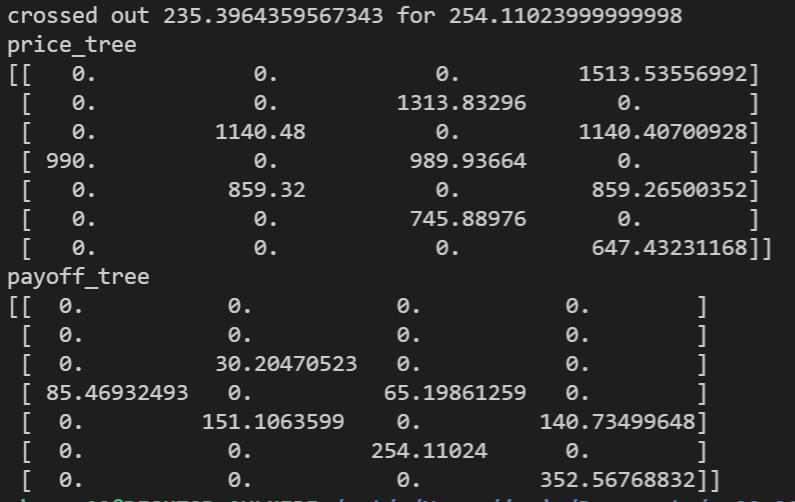
\includegraphics[width=120mm]{./2a.png}
\end{figure}

\subsection*{(b)}

As we compare, we can see that the starting node's value differs by $\sim 85.46932493 - \sim 81.452947 = $ \framebox[1.1\width]{$\mathbf{\sim \$ 4.01637793}$}

\begin{figure}[h]
  \centering
  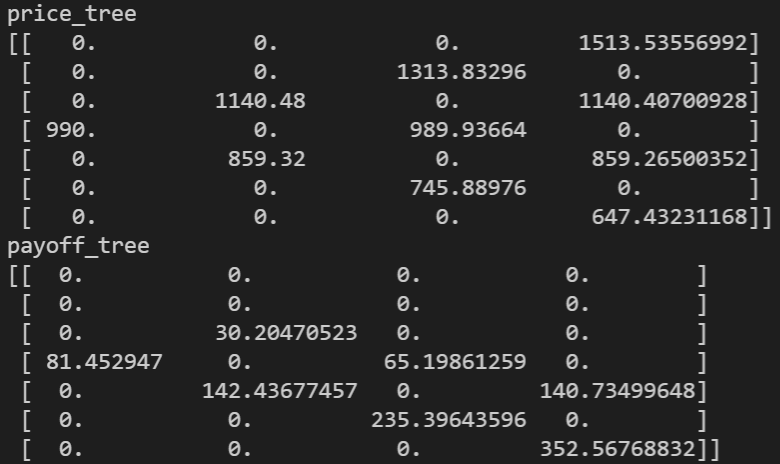
\includegraphics[width=120mm]{./2b.png}
\end{figure}

\subsection*{(c)}

Suppose we chop the same time to expiration up into much smaller time steps for this binomial lattice, and we find the price for 149 time steps to 84, 150 time steps to be 85, and 151 time steps to be 86. What should we take as the option premium in this case?



\newpage
}

\section*{3.}
{\Large 

\framebox[1.1\width]{\textbf{answer}}

Amazon's stock price is \$3200 on Monday, 7 June 2021 (today). It pays no divdend. The current annual risk-free rate is 1\%, and the annual stock price volatility is 30\%.

\subsection*{(a)}

Using the Black-Scholes pricing model, and the European 30/360 day count-adjusted year fraction, what is the premium for a European call option on Amazon stock expiring on 30 June 2021 with a strike of \$3150? (You may use your 30/360-EUR function from Assignment 2)

\subsection*{(b)}

What is the price of an American option with the same market and product data, and the same day-count?

\subsection*{(c)}

What is the price of a corresponding European put option?



\newpage
}

\section*{4.}
{\Large 

\subsection*{(a)}
We know that with $t_0 = 0$, $P(t, T) = P(0, T) / P(0, t)$, or that \\
$P(0, T) = P(t, T) \cdot P(0, t)$: \\ \\
$P(T_0, T_2) = P(T_1, T_2) \cdot P(T_0, T_1) = 0.940 \cdot 0.950 = $ \framebox[1.1\width]{$\mathbf{0.893}$} \\ 
$P (T_0, T_3) = P(T_2, T_3) \cdot P(T_0, T_2) = 0.932 \cdot 0.893 = $ \framebox[1.1\width]{$\mathbf{0.832276}$} \\
$P(T_0, T_4) = P(T_3, T_4) \cdot P(T_0, T_3) = 0.925 \cdot 0.832276 = $ \framebox[1.1\width]{$\mathbf{0.7698553}$} \\
$P(T_0, T_5) = P(T_4, T_5) \cdot P(T_0, T_4) = 0.919 \cdot 0.7698553 = $ \framebox[1.1\width]{$\mathbf{0.7074970207}$} \\
$P(T_0, T_6) = P(T_5, T_6) \cdot P(T_0, T_5) = 0.913 \cdot 0.7074970207 =  $ \framebox[1.1\width]{$\mathbf{0.64594477989}$}

\subsection*{(b)}

Since each discount rate is annual, we know that the year-count difference between any two adjacent $T_i$ is 1, and adapt this accordingly between $T_0$ and $T_i$: \\ $R(t, T) := -ln(P(t, T)) / \tau(t, T)$ \\ \\
$R(T_0, T_1) = -ln(P(T_0, T_1)) / \tau(T_0, T_1) = -ln(0.950) / 1 = $ \framebox[1.1\width]{$\mathbf{0.05129329438}$} \\
$R(T_0, T_2) = -ln(P(T_0, T_2)) / \tau(T_0, T_2) = -ln(0.893) / 2 = $ \framebox[1.1\width]{$\mathbf{0.05658434905}$} \\
$R(T_0, T_3) = -ln(P(T_0, T_3)) / \tau(T_0, T_3) = -ln(0.832276) / 3 = $ \framebox[1.1\width]{$\mathbf{0.06119705413}$} \\
$R(T_0, T_4) = -ln(P(T_0, T_4)) / \tau(T_0, T_4) = -ln(0.7698553) / 4 = $ \framebox[1.1\width]{$\mathbf{0.06538817596}$} \\
$R(T_0, T_5) = -ln(P(T_0, T_5)) / \tau(T_0, T_5) = -ln(0.7074970207) / 5 = $ \framebox[1.1\width]{$\mathbf{0.06920437209}$} \\
$R(T_0, T_6) = -ln(P(T_0, T_6)) / \tau(T_0, T_6) = -ln(0.64594477989) / 6 = $ \framebox[1.1\width]{$\mathbf{0.07284020981}$} \\


}

\end{document}